\section{Phase framework and local geometry}
\label{core:framework}

To deform the local geometry while preserving an orthonormal measurement, we put the tunable parameters in a diagonal phase. For $n\ge2$, we use the computational basis $\ket{z_1\cdots z_n}$, with $z_j\in\mathbb F_2$, and the circuit convention of Ref.~\cite{PauwelsGisin2026}. Products act from right to left. Write
\begin{align}
 C_n&=S(n)H_n,\qquad M[D]=C_nDH^{\otimes n},\nonumber\\
 S(n)&=\mathrm{CNOT}_{2\to1}\cdots\mathrm{CNOT}_{n\to n-1},
 \label{core:phase-family}
\end{align}
where $H_n$ acts only on the last qubit and $D$ is diagonal with unit-modulus entries. By unitarity, the columns $\ket{\psi_k}=M[D]\ket{k}$ form a complete orthonormal measurement for every such $D$. Their local geometry is determined by the seed $\ket{\psi_0}$: writing $k=(e_1,\ldots,e_{n-1},\sigma)$ with $e\in\mathbb F_2^{n-1}$ and $\sigma\in\mathbb F_2$, the columns obey the exact Pauli orbit identity
\begin{equation}
 \ket{\psi_{e,\sigma}}=
 \left[\prod_{h=1}^{n-1}(Z_hZ_{h+1})^{e_h}\right]
 (X^{\otimes n})^\sigma\ket{\psi_0}.
 \label{core:orbit}
\end{equation}
This orbit propagates the seed's local Bloch vectors to all columns. To obtain regular tetrahedra with a common radius, it suffices to make the seed's signed local components equal. Our local coordinates are fixed throughout: only the final-qubit $Y$ component is sign-adjusted, $\widetilde Y_n=-Y_n$; every other $\widetilde P$ equals the corresponding physical Pauli operator. A common signed component $m\ge0$ therefore means seed Bloch vectors $m(1,1,1)$ for $j<n$ and $m(1,-1,1)$ for $j=n$.

We deform the reference phase
\begin{equation}
 \begin{aligned}
 f_0(z)&=\sum_{\ell=2}^n(-1)^\ell e_\ell(z)\\
 &=\begin{cases}0,&z=0,\\ |z|-1,&z\ne0,\end{cases}\pmod4.
 \end{aligned}
 \label{core:reference-phase}
\end{equation}
where $e_\ell$ is the elementary symmetric polynomial and $|z|$ is the Hamming weight. The reference measurement has $D_0(z)=i^{f_0(z)}$ and radius
\begin{equation}
 c_n=2^{1-n},\qquad r_E(n)=\sqrt3\,c_n.
 \label{core:reference-radius}
\end{equation}

To compute the seed's signed components, we separate a background state from a correction at the physical zero string. For any real function $\Theta$ on $\mathbb F_2^n$, set
\begin{align}
 \ket{\chi_\Theta}&=2^{-n/2}\sum_z i^{|z|}e^{i\Theta(z)}\ket z,\nonumber\\
 D_\Theta(z)&=\begin{cases}1,&z=0,\\
 i^{f_0(z)}e^{i\Theta(z)},&z\ne0.
 \end{cases}
 \label{core:background}
\end{align}
The seed is exactly
\begin{equation}
 \ket{\psi_0}=-iC_n\left[\ket{\chi_\Theta}
 +2^{-n/2}\big(i-e^{i\Theta(0)}\big)\ket{0^n}\right].
 \label{core:defect-state}
\end{equation}
The correction changes one physical input amplitude, irrespective of how $\Theta$ is represented.

\begin{lemma}[Local phase mechanism]
\label{core:mechanism}
For a signed local Pauli operator, write
\begin{equation}
 R=C_n^\dagger\widetilde P C_n=i^kX^aZ^b,\quad
 h=a\oplus b,\quad\Gamma=i^{k-|a|},
 \label{core:pauli-notation}
\end{equation}
and $B_R=\bra{\chi_\Theta}R\ket{\chi_\Theta}$. Then
\begin{equation}
 \langle\widetilde P\rangle
 =B_R+c_n\operatorname{Re}\!\left[
 \Gamma e^{-i\Theta(a)}\big(i-e^{i\Theta(0)}\big)\right].
 \label{core:signal}
\end{equation}
If all these signed expectations equal $m\ge0$, every measurement column has a true one-qubit reduced state
\begin{equation}
 \rho_{j,e,\sigma}
 =\frac12\left[I+\sqrt3m\,\mathbf v_{j,\kappa_j,\sigma}
 \cdot\boldsymbol\sigma\right],
 \label{core:bloch-orbit}
\end{equation}
where $e_0=e_n=0$, $\kappa_j=e_{j-1}\oplus e_j$, and
\begin{equation}
 \begin{aligned}
 \mathbf v_{j,q,s}&=\frac1{\sqrt3}
 \big((-1)^q,\epsilon_j(-1)^{q+s},(-1)^s\big),\\
 \epsilon_j&=\begin{cases}1,&j<n,\\-1,&j=n.\end{cases}
 \end{aligned}
 \label{core:vertices}
\end{equation}
For each $j$, these four unit vectors form a regular tetrahedron, and each label $(q,s)$ occurs $2^{n-2}$ times.
\end{lemma}

All pullbacks have $a\ne0$, so the correction in Eq.~\eqref{core:defect-state} has no diagonal contribution to a local expectation. Its two cross terms give Eq.~\eqref{core:signal}. Conjugation by the orbit operators in Eq.~\eqref{core:orbit} gives the tetrahedral signs in Eq.~\eqref{core:vertices}. Appendix~\ref{core:appendix} gives the pullbacks and the reduced-state derivation.

For the Boolean phase $\Theta=tq$, $q(0)=1$, the pullbacks fall into two classes: class I has $\Gamma=-i$ and $h\cdot a=1$, while class II has $\Gamma=-1$ and $h\cdot a=0$. With normalized Walsh coefficients
\begin{equation}
 \begin{aligned}
 W_q(h)&=2^{-n}\sum_z(-1)^{q(z)\oplus h\cdot z},\\
 D_aq(z)&=q(z)\oplus q(z\oplus a).
 \end{aligned}
 \label{core:walsh-def}
\end{equation}
the background is
\begin{equation}
 B_R(t)=\begin{cases}
 -\sin t\,W_q(h),&\text{class I},\\
 -\sin^2(t/2)\,W_{D_aq}(h),&\text{class II}.
 \end{cases}
 \label{core:boolean-background}
\end{equation}
These formulas express the background in terms of Walsh coefficients of the phase function and its derivatives.

\section{A unified family for all \texorpdfstring{$n\ge5$}{n >= 5}}
\label{core:unified}

Equation~\eqref{core:signal} suggests two design requirements: cancel every background term $B_R(t)$, and make the remaining cross terms equal. For Boolean phases, the first requirement gives the Walsh cancellations in Eq.~\eqref{core:boolean-background}, while the second fixes the values $q(a)$ at the local flips. For every integer $n\ge5$, four linear features reduce these requirements to conditions on one fixed four-bit kernel. Define the two internal parity blocks
\begin{equation}
 \begin{aligned}
 E_n&=\{2,4,\ldots\}\cap[2,n-2],\\
 O_n&=\{3,5,\ldots\}\cap[2,n-2],
 \end{aligned}
\end{equation}
and the four linear features
\begin{align}
 x&=z_1\oplus z_{n-1},& b&=\bigoplus_{j\in E_n}z_j,\nonumber\\
 c&=\bigoplus_{j\in O_n}z_j,& s&=z_1\oplus z_n.
 \label{core:features}
\end{align}
Write $\mathcal L_nz=(x,b,c,s)$. Both internal blocks are nonempty; the four features are independent. On $\mathbb F_2^4$, take
\begin{equation}
 F(x,b,c,s)=\begin{cases}
 1\oplus(1\oplus c)(x\oplus b),&s=0,\\
 b\oplus xc,&s=1.
 \end{cases}
 \label{core:kernel}
\end{equation}
Define
\begin{equation}
 q_n(z)=F(\mathcal L_nz),\qquad
 d_n(z)=q_n(z)-\delta_{z,0}.
 \label{core:support}
\end{equation}
Here the subtraction is in the integers. Since $F(0)=1$, $d_n$ is still Boolean. Only the physical zero string is removed, not the whole fiber $\mathcal L_nz=0$.

Figure~\ref{fig:unified}(a) shows how the same four-feature kernel determines the phase at every $n\ge5$; panel (b) displays the resulting radius in units of $r_E(n)$.
\begin{figure*}[tbp]
  \centering
  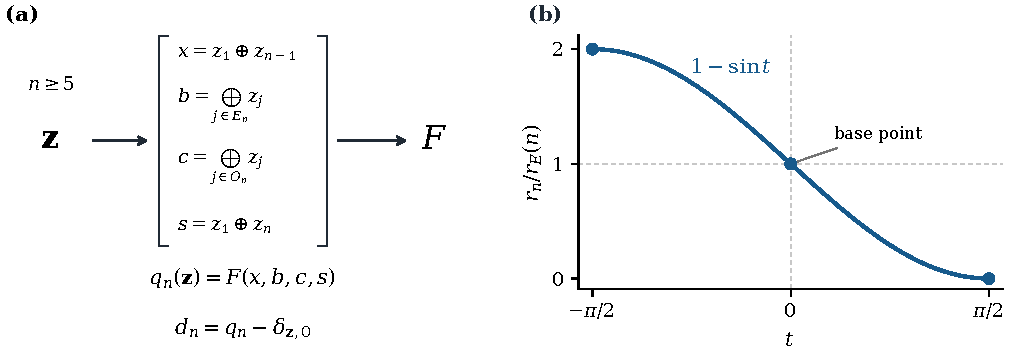
\includegraphics[width=\textwidth]{figures/fig1_unified.pdf}
  \caption{Unified phase deformation for every $n\geq5$.
  (a) Four linear Boolean features feed the same kernel $F$; the only removed support point is the physical string $\mathbf z=0$.
  The blocks $E_n$ and $O_n$ contain the even and odd indices in $[2,n-2]$, respectively.
  (b) The normalized common Bloch radius $r_n(t)/r_E(n)=1-\sin t$ on $[-\pi/2,\pi/2]$, where $r_E(n)=\sqrt3/2^{n-1}$ is the reference radius.
  From left to right, the marked points give the enhanced endpoint, the specified EJM at $t=0$, and the endpoint with maximally mixed one-qubit marginals.}
  \label{fig:unified}
\end{figure*}

\begin{theorem}[Unified enhanced family]
\label{core:unified-theorem}
For every integer $n\ge5$, let
\begin{equation}
 D_{n,t}(z)=i^{f_0(z)}e^{itd_n(z)},\qquad
 M_n(t)=C_nD_{n,t}H^{\otimes n}.
 \label{core:unified-measurement}
\end{equation}
For every real $t$, its columns are an orthonormal basis, and their one-qubit reduced states are Eq.~\eqref{core:bloch-orbit} with
\begin{equation}
 m_n(t)=c_n(1-\sin t),\qquad
 r_n(t)=r_E(n)(1-\sin t).
 \label{core:radius}
\end{equation}
The tetrahedral directions are independent of $t$. On
\begin{equation}
 J=[-\pi/2,\pi/2],\qquad r_n(J)=[0,2r_E(n)],
 \label{core:interval}
\end{equation}
the radius is continuous and strictly decreasing. At $t=0$, the reference measurement is recovered column by column; at $t=-\pi/2$ the radius is $2r_E(n)$, and at $t=\pi/2$ every one-qubit reduced state is $I/2$.
\end{theorem}

\begin{proof}
The proof separates the dimension-dependent feature map from six fixed four-bit cancellations. First, any sum of the form
\begin{equation}
 2^{-n}\sum_z(-1)^{h\cdot z}G(\mathcal L_nz)
 \label{core:pairing-sum}
\end{equation}
vanishes when $h$ is outside the row space of $\mathcal L_n$: a translation $z\mapsto z\oplus w$ with $\mathcal L_nw=0$ and $h\cdot w=1$ reverses each summand's sign. Inside that row space, write $h=\mathcal L_n^TH$. Equal fiber sizes reduce Eq.~\eqref{core:pairing-sum} to $2^{-4}\sum_v(-1)^{H\cdot v}G(v)$. The same argument applies to a derivative of $q_n$, since $D_aq_n=(D_AF)\circ\mathcal L_n$ with $A=\mathcal L_na$.

Second, the local characters in the pullback table leave only
\begin{align}
 W_F(9)&=W_F(11)=W_F(15)=0,\nonumber\\
 W_{D_6F}(6)&=W_{D_7F}(13)=W_{D_7F}(11)=0.
 \label{core:six-cancellations}
\end{align}
Integers encode $(x,b,c,s)$ with $x$ the most significant bit; the Walsh normalization is $2^{-4}$. The six sums vanish by pairing over feature bits. Appendix~\ref{core:alln-classification} gives the finite calculation and proves that these six identities cover every local component for all $n\ge5$, including the additional residual terms at $n=5,6,7$. Equation~\eqref{core:boolean-background} therefore gives $B_R(t)=0$ identically.

Third, every class-I flip satisfies $F(\mathcal L_na)=0$, and every class-II flip satisfies $F(\mathcal L_na)=1$. Equation~\eqref{core:signal} therefore reduces, respectively, to
\begin{align}
 c_n\operatorname{Re}[-i(i-e^{it})]&=c_n(1-\sin t),\nonumber\\
 c_n\operatorname{Re}[-e^{-it}(i-e^{it})]&=c_n(1-\sin t).
\end{align}
Lemma~\ref{core:mechanism} transfers this seed identity to all measurement columns. The endpoint, base-point, and image statements follow from the diagonal phase and the strict monotonicity of $\sin t$ on $J$.
\end{proof}

The enhancement has a direct one-qubit entanglement interpretation. All outcomes and all $1|(n-1)$ cuts share the spectrum
\begin{equation}
 \lambda_\pm=\frac{1\pm r_n(t)}2,
 \qquad \operatorname{Tr}\rho_j^2=\frac{1+r_n(t)^2}{2}.
 \label{core:spectrum}
\end{equation}
Their entropy is $h_2((1+r_n(t))/2)$, where $h_2(p)=-p\log_2p-(1-p)\log_2(1-p)$ with its continuous endpoint values. Increasing the Bloch radius decreases this bipartite entanglement. At $t=\pi/2$, the point correction in Eq.~\eqref{core:defect-state} vanishes; at $t=-\pi/2$, its interference produces twice the reference local signal. Four linear features suffice to express the phase for all $n$, while the feature extraction itself still depends on the physical register size.





